\begin{figure}[H]
	\begin{center}
		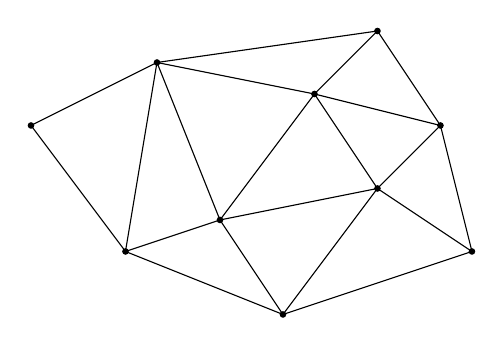
\begin{tikzpicture}[scale=0.4]
		%\draw [<->,thick] (0,10) node (yaxis) [left] {}
		%|- (15,0) node (xaxis) [below] {};
		%centroids
		\fill ( 2, 7) circle (3pt);
		\fill ( 5, 3) circle (3pt);
		\fill ( 6, 9) circle (3pt);
		\fill ( 8, 4) circle (3pt);
		\fill (10, 1) circle (3pt);
		\fill (11, 8) circle (3pt);
		\fill (13, 5) circle (3pt);
		\fill (13,10) circle (3pt);
		\fill (15, 7) circle (3pt);
		\fill (16, 3) circle (3pt);
		
		
		\draw [-] ( 2,7) -- ( 6,9);
		\draw [-] ( 6,9) -- ( 5,3);
		\draw [-] ( 5,3) -- ( 2,7);
		\draw [-] ( 6,9) -- ( 8,4);
		\draw [-] (10,1) -- ( 8,4);
		\draw [-] ( 5,3) -- (10,1);
		\draw [-] ( 8,4) -- ( 5,3);
		\draw [-] ( 8,4) -- (11,8);
		\draw [-] (11,8) -- (6,9);
		\draw [-] ( 6,9) -- (13,10);
		\draw [-] (11,8) -- (13,10);
		\draw [-] (15,7) -- (13,10);
		\draw [-] (16,3) -- (15,7);
		\draw [-] (16,3) -- (10,1);
		\draw [-] (16,3) -- (13,5);
		\draw [-] (13,5) -- (15,7);
		\draw [-] (13,5) -- (10,1);
		\draw [-] (13,5) -- (8,4);
		\draw [-] (13,5) -- (11,8);
		\draw [-] (15,7) -- (11,8);
		\end{tikzpicture}
	\end{center}
	\caption{Example of a Delaunay Triangulation}
	\label{fig:dt1}
\end{figure}